\documentclass[12pt]{ctexart}

% 包含必要的包
\usepackage[utf8]{inputenc}
\usepackage{amsmath, amssymb}  % 数学符号包
\usepackage{graphicx}  % 插入图片的包
\usepackage{hyperref}  % 生成超链接
\usepackage{fancyhdr}  % 页眉页脚设置
\usepackage{geometry}  % 页面设置
\usepackage{titlesec}  % 用于自定义 section 的格式
\usepackage{float}
\geometry{a4paper, margin=1in}

\titleformat{\section}[hang]{\normalfont\Large\bfseries}{\thesection}{1em}{}


% Header and footer
\setlength{\headheight}{14.49998pt}
\addtolength{\topmargin}{-2.49998pt}

\pagestyle{fancy}
\fancyhf{}
\fancyhead[L]{《统计信号处理》实验报告}
% \fancyhead[M]{清华大学}
\fancyhead[R]{刘昱杉 2024214103}
\fancyfoot[C]{\thepage}



\begin{document}

\begin{titlepage}
    \begin{center}
        % Insert logo
        
\includegraphics[width=5cm]{tsinghua_logo.png}\\[4cm]  % 插入图标并设置下方间距
        {\Huge 实验一:信号检测与分类} \\[4cm]
        {\large 刘昱杉  \ \  2024214103}\\[6cm]
        {\normalsize \today}\\[1cm]
        \vfill
        \text{注:本实验报告为单人独立完成}\\
        \text{关于本实验报告对应的源码 详见\texttt{code}目录下\texttt{Task\_i}所对应文件}

    \end{center}
\end{titlepage}

\section*{一、单次电平信号检测}

\subsection*{1. 实验内容}
在本次实验中,我们设计了这样一个系统:信号产生方产生一个单电平信号,并叠加一个均值为0,方差为\(\sigma_n^2\)的高斯噪声;
信号检测方接收到这个信号,通过二元假设来对信号的电平进行判决:

\begin{itemize}
    \item 假设 \( H_0 \):仅存在噪声 \( z = n \)。
    \item 假设 \( H_1 \):信号叠加噪声 \( z = A + n \)。
\end{itemize}

检测方法选用阈值检测,设定检测阈值\(\gamma\),以检测统计量 \( z \) 是否超过阈值来判断假设:

\begin{itemize}
    \item 若 \( z > \gamma \),则判定 \( H_1 \) 成立。
    \item 若 \( z \leq \gamma \),则判定 \( H_0 \) 成立。
\end{itemize}

我们知道,在假设噪声 \( n \) 服从高斯分布 \( N(0, \sigma_n^2) \) 的情况下,观测值 \( z \) 在不同假设下的分布为:
\begin{itemize}
    \item 假设 \( H_0 \) 下:\( z \sim N(0, \sigma_n^2) \)。
    \item 假设 \( H_1 \) 下:\( z \sim N(A, \sigma_n^2) \)。
\end{itemize}

则检测率 \( P_D \) 和误警率 \( P_{FA} \) 可分别表示为:
\[
P_D = P(z > \gamma | H_1) = Q\left(\frac{\gamma - A}{\sigma_n}\right)
\]
\[
P_{FA} = P(z > \gamma | H_0) = Q\left(\frac{\gamma}{\sigma_n}\right)
\]
其中,\( Q(x) \) 是标准正态分布右尾的累积分布函数。根据公式可以看出,随着 \( A \) 或 SNR 增加,分布的重叠区域减少,导致检测性能提升。

在本实验中,我们生成的数据主要包含:

\begin{enumerate}
    \item 在假设 \( H_0 \) 下生成的噪声数据 \( z = n \)。
    \item 在假设 \( H_1 \) 下生成的信号加噪声数据 \( z = A + n \)。
\end{enumerate}

每种实验条件下生成 1000 个数据点,计算不同条件下的检测性能。

\subsection*{2. 实验结果}

1. ROC曲线:实验结果绘制了在不同信噪比(SNR)和信号电平A下的ROC曲线,如图1所示。可以看到,在SNR增加时,ROC曲线逐渐接近左上角,在信号电平A增加时,ROC曲线也逐渐向左上角移动,二者的改变都可以使得检测性能提升。

\begin{figure}[H]
    \centering
    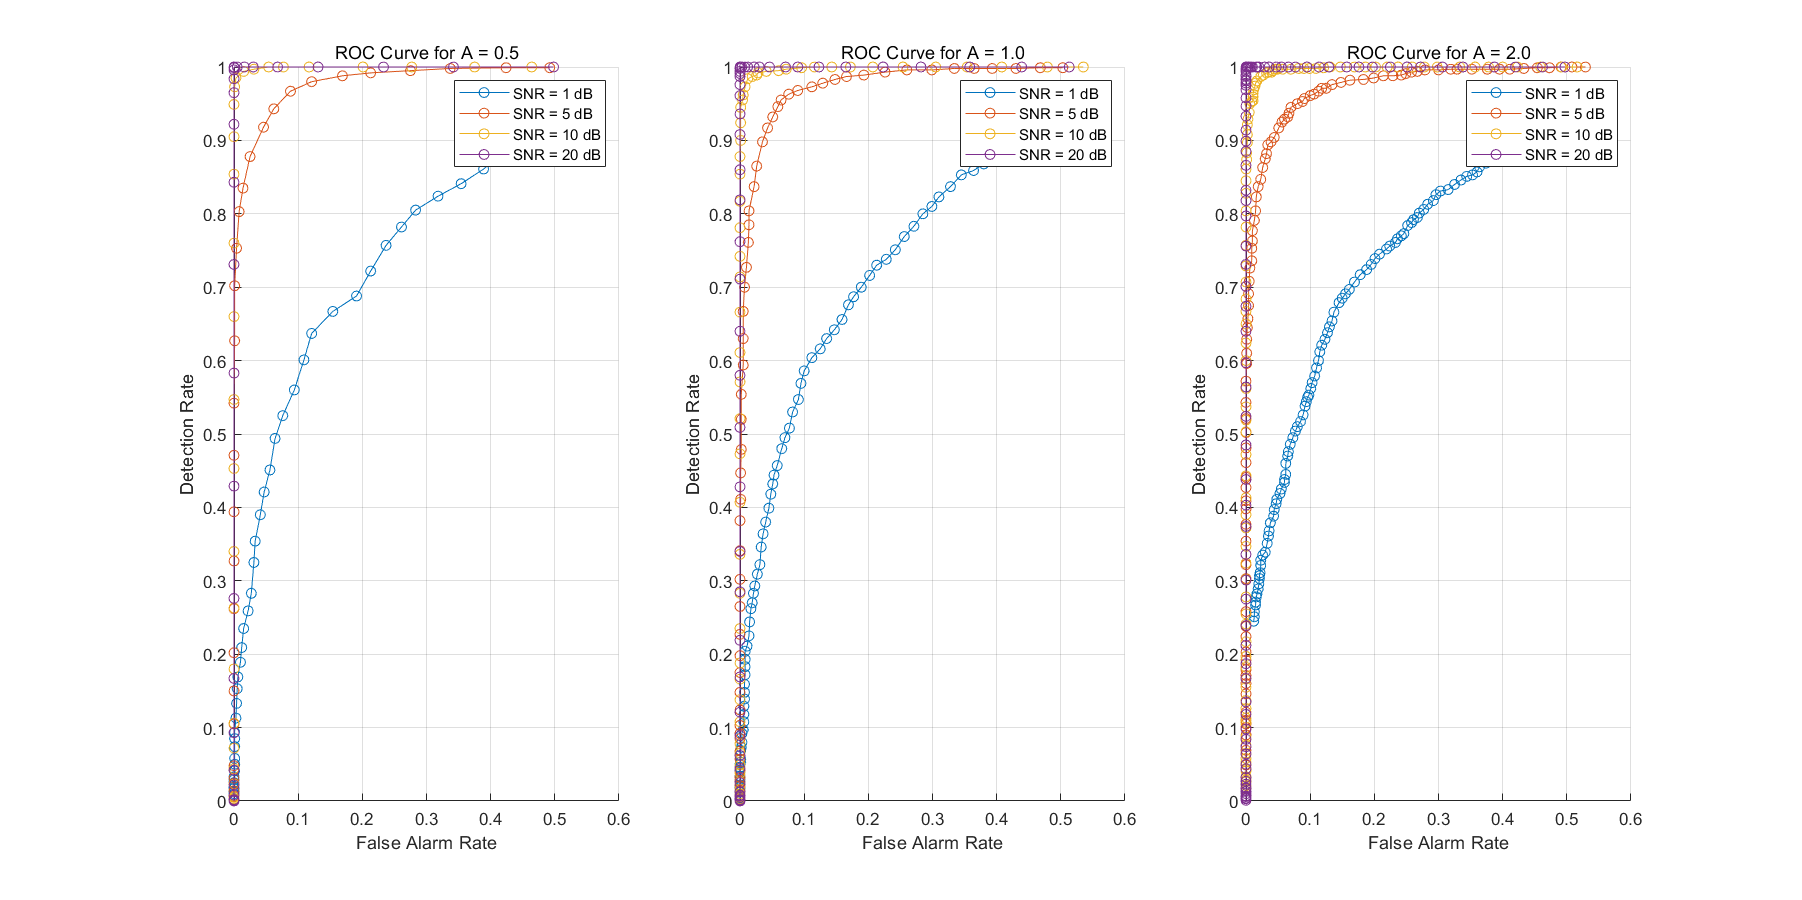
\includegraphics[width=0.85\textwidth]{image/output1.png}
    \caption{不同信噪比和信号电平下的 ROC 曲线}
    \label{fig:roc}
\end{figure}

2. 检测率和误警率:绘制了在不同信噪比(SNR)和信号电平A下的检测率和误警率,如图2所示。可以看到,随着SNR和A的增加,检测率逐渐增加,误警率逐渐减小,检测性能逐渐提升。

\begin{figure}[H]
    \centering
    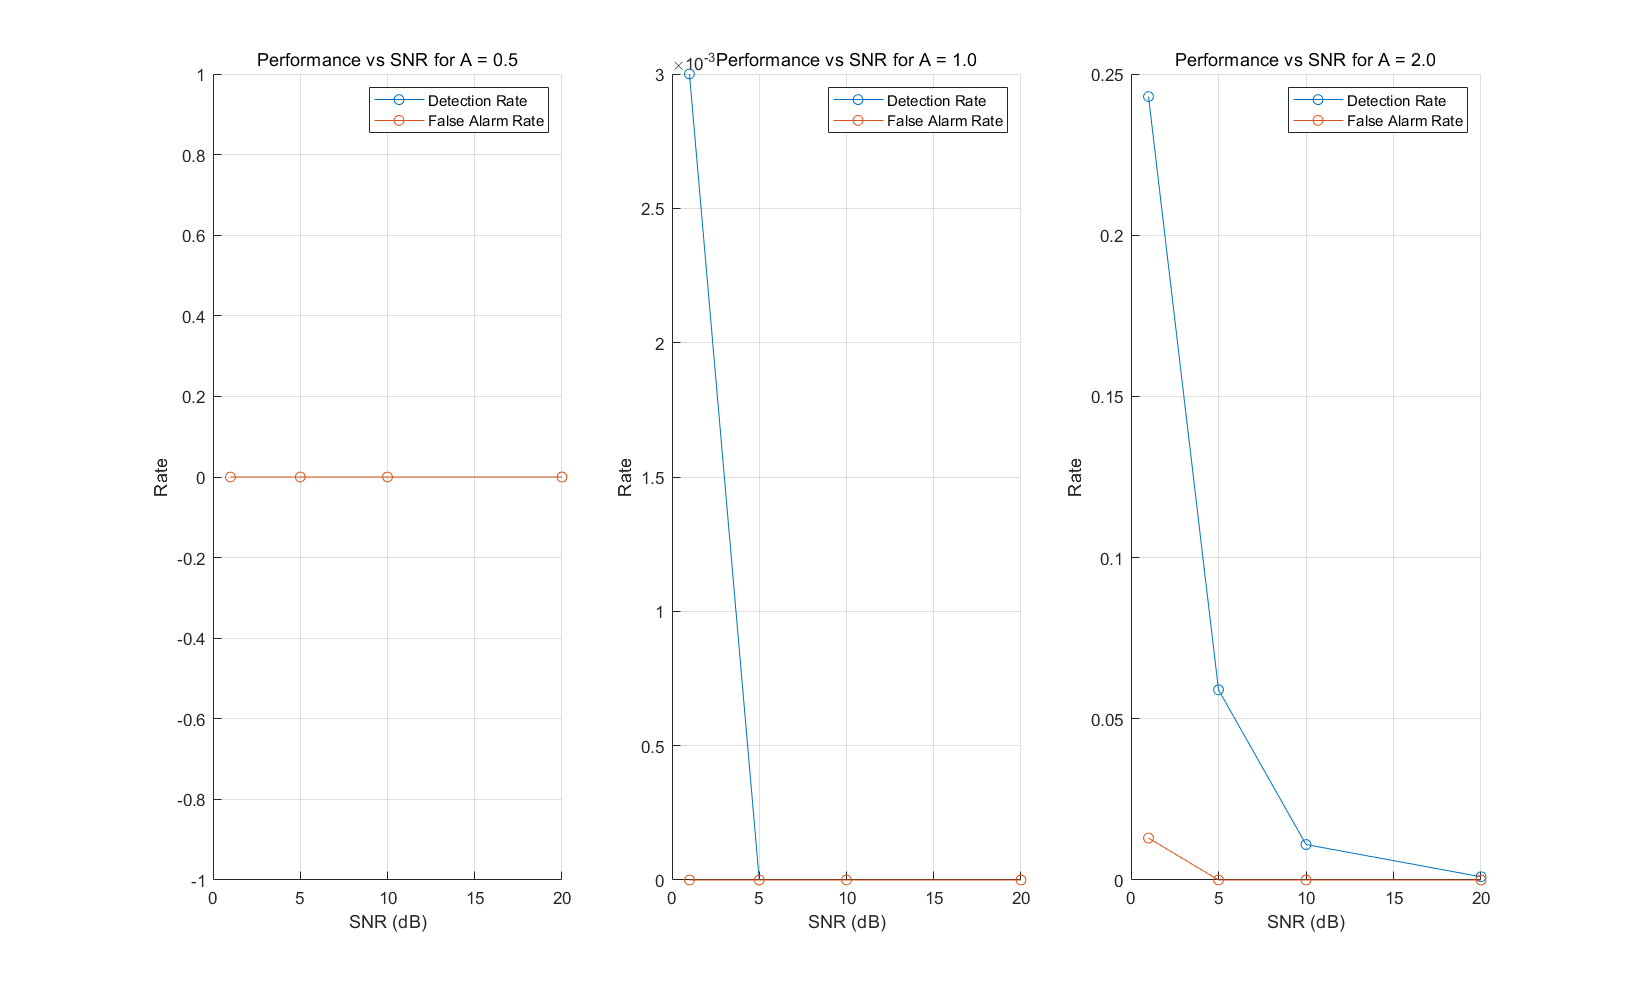
\includegraphics[width=0.85\textwidth]{image/output2.png}
    \caption{不同信噪比和信号电平下的检测率和误警率}
    \label{fig:pd_pfa}

\end{figure}

\subsection*{3. 实验分析}
\begin{itemize}
    \item \textbf{SNR 对检测性能的影响}:随着 SNR 的增加,信号与噪声的差异变得更加显著。检测器在相同的阈值下更容易区分信号和噪声,导致检测率提升,误判率下降。ROC 曲线表现为向左上角靠近,表明检测性能得到显著提升。
    \item \textbf{信号电平 \( A \) 对检测性能的影响}:增大信号电平 \( A \) 使得 \( H_1 \) 下的分布与 \( H_0 \) 下的分布差异更显著,在较低阈值下也能保持较高的检测率和较低的误警率。
    \item \textbf{误警率与检测率的权衡}:选择不同的阈值可以实现误警率与检测率之间的平衡。
\end{itemize}

实验结果表明,在较高的 SNR 和信号电平 \( A \) 下,接收机的检测性能可以得到显著提升。这验证了 SNR 和信号电平对于信号检测的重要性。在实际应用中,可以通过增加信号强度或提升信噪比来优化检测器的性能。

\section*{二、恒定值连续信号的多次观测}

\subsection*{1. 实验内容}

在本次实验中,我们设计了这样一个系统:信号产生方产生一个恒定值信号 \( A \),并叠加一个均值为0,方差为\(\sigma_n^2\)的高斯噪声;
通过改变观测次数 \( N \),计算不同观测点数下的误差概率\(P_e\),进而验证观测点数量对检验准确性的影响。

系统的假设模型如下:

\begin{itemize}
    \item 假设 \( H_0 \):仅包含噪声的信号,表示为 \( z = n \)。
    \item 假设 \( H_1 \):包含信号和噪声的信号,表示为 \( z = A + n \),其中 \( A \) 为已知信号电平。
\end{itemize}

我们设置信号电平\(A=1\),噪声标准差\(\sigma = 1\)。通过不同的观测点数\(N\)(从1到50,间隔为2),以分析接收机性能随观测点书的变化。
同时,阈值检测器的检测阈值\(\gamma = A/2\),并基于判别阈值来判断观测结果。每个观测点数下重复1000次进行多次实验,并计算平均误差概率作为当前观测点数对应的误差概率\(P_e\)。

\subsection*{2. 实验结果}

通过不同观测点数下的实验,得到观测点数 \( N \) 与误差概率 \( P_e \) 的关系曲线,结果如下:

\begin{itemize}
    \item 随着观测点数 \( N \) 的增加,误差概率 \( P_e \) 逐渐降低。这表明,增加观测点数有助于提升接收机的检测准确度。
    \item 当观测点数较少时,信号和噪声的区分度较低,误判概率较高;而随着观测点数增加,检测器能够更好地估计信号的平均值,使得 \( H_0 \) 和 \( H_1 \) 下的分布更易分离,从而降低误判率。
\end{itemize}

\begin{figure}[H]
    \centering
    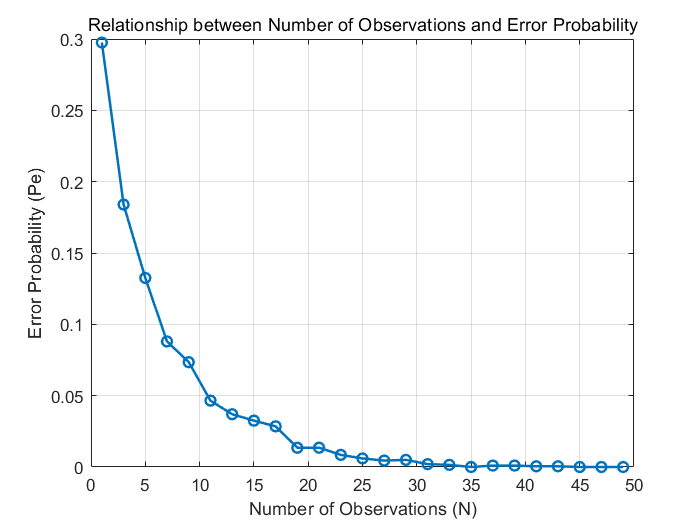
\includegraphics[width=0.8\textwidth]{image/output3.png}
    \caption{观测点数 \( N \) 与误差概率 \( P_e \) 的关系曲线}
\end{figure}

\subsection*{3. 实验分析}

\begin{itemize}
    \item \textbf{观测点数对检测性能的影响}:实验结果表明,观测点数 \( N \) 增加有助于降低误差概率 \( P_e \)。这是因为更多的观测点数能够提供更多的信息,使得平均值计算更接近真实信号,增强了检测的稳健性。
    \item \textbf{误差概率的收敛性}:从曲线中可以观察到,当 \( N \) 增加到一定程度时,误差概率趋于平稳,表明观测点数的进一步增加对误判概率的改善效果有限。
\end{itemize}


\section*{三、最佳接收机设计}

\subsection*{1. 实验内容}

本实验旨在设计并分析三种常用调制方式(CPSK、CFSK 和 CASK)的最佳接收机性能,研究其在加性高斯白噪声(AWGN)信道下的误码概率(Pe)随信噪比(SNR)的变化。

三种调制方式的误码概率公式分别为:

\begin{itemize}
    \item \textbf{CPSK:} $P_e = Q\left( \sqrt{2 \cdot \frac{E_b}{N_0}} \right)$
    \item \textbf{CFSK:} $P_e = Q\left( \sqrt{\frac{E_b}{N_0}} \right)$
    \item \textbf{CASK:} $P_e = Q\left( \sqrt{\frac{E_b}{2N_0}} \right)$
\end{itemize}

具体实现中,我们设置SNR的范围从0到20dB,步长为0.5dB,并计算各种调制方式在不同SNR下的误码概率。
其中,对于CPSK,我们将比特'0'与'1'映射为符号-1和+1;对于CFSK,分别用两种频率的正交信号\(s_0(t)\)和\(s_1(t)\)来对应比特'0'和'1';对于CASK信号,分别将比特'0'和'1'映射为幅度0和\(\sqrt{2E_s}\)。
对于信道建模,分别在调制信号中加入加性高斯白噪声,模拟噪声的影响。

接收机设计方面:对于CPSK,我们使用相干检测,通过比较接收信号和0的大小来进行判决;对于CFSK,通过设计匹配滤波器,依据更大的输出进行判决;对于CASK,通过与阈值比较接收信号进行相干检测判决。
通过比较检测出的比特和原始发送的比特,计算误码率\(P_e\),并绘制在对数坐标下。

\subsection*{2. 实验结果}
实际仿真曲线如下图所示:

\begin{figure}[H]
    \centering
    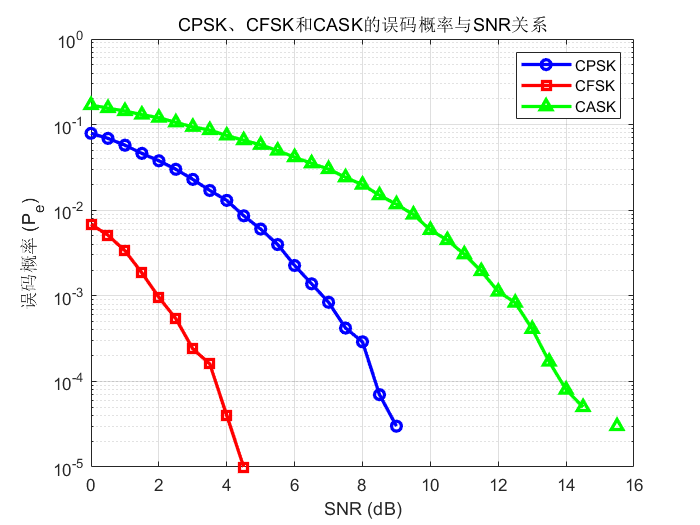
\includegraphics[width=0.8\textwidth]{image/output4-1.png}
    \caption{不同调制方式的误码概率随 SNR 的变化}
\end{figure}

\begin{itemize}
    \item \textbf{CPSK}:在相同 SNR 下,CPSK 的误码概率最低。由于其符号之间的欧氏距离较大,因此抗噪能力较强。CPSK 对于 AWGN 的抑制能力最好,适合在噪声环境较大的场景中应用。
    \item \textbf{CFSK}:CFSK 的误码概率高于 CPSK,但低于 CASK。其性能介于 CPSK 和 CASK 之间,适合对抗噪声性能要求适中的场景。相干 FSK 在频率域上通过正交信号实现二进制数据的调制,与 CPSK 相比误码概率稍高,但由于不依赖幅度,能在非理想的幅度抖动环境中稳定工作。
    \item \textbf{CASK}:CASK 的误码概率最高,其抗噪性能相对较差。在 AWGN 信道中,CASK 对幅度噪声较为敏感,因此误码率随 SNR 增长的下降趋势相对较慢。这种调制方式适合噪声较低的通信场景,但在高噪声环境中不具优势。
\end{itemize}

\subsection*{3. 实验分析}

\begin{itemize}
    \item 在相同的信噪比条件下,CPSK 的抗噪性能最优,其次是 CFSK,最后是 CASK。
    \item CPSK 的高抗噪性源于相位键控符号间的较大欧氏距离,使得信号间的区分度增加,从而在接收机端实现更好的误码率性能。
    \item CASK 的误码概率受噪声影响较大,表现出明显的性能劣势,因此在高噪声环境下应优先选择 CPSK 或 CFSK。
\end{itemize}

\section*{四、随幅随相信号检测}

\subsection*{1. 实验内容}

本实验旨在研究随附随想信号与随想信号的检测性能差异,通过分别比较其在不同检测概率下的信噪比需求,进而分析其抗噪声性能。
在随机信号检测中,信号的检测性能受到信号幅度和相位变化的影响。本实验研究两种信号模型:

\begin{itemize}
    \item \textbf{随相信号}:幅度固定且已知,相位是随机的。接收信号模型为:
    \begin{itemize}
        \item 假设 \( H_0 \):仅有噪声 \( n(t) \),即 
        \[ z(t) = n(t) \]
        \item 假设 \( H_1 \):有幅度为 \( A \) 的信号和随机相位 \( \varphi \) 加上白噪声,即 
        \[ z(t) = A \sin(\omega_0 t + \varphi) + n(t) \]
    \end{itemize}

    \item \textbf{随幅随相信号}:幅度和相位均为随机,接收信号模型为:
    \begin{itemize}
        \item 假设 \( H_0 \):仅有噪声 \( n(t) \),即 \[ z(t) = n(t) \]
        \item 假设 \( H_1 \):随机幅度 \( A \) 和随机相位 \( \varphi \) 的信号加白噪声,即 \[ z(t) = A \sin(\omega_0 t + \varphi) + n(t) \]
    \end{itemize}

    在此模型中,幅度 $A$ 服从已知的随机分布,假设服从均匀分布。
\end{itemize}

实验具体可分为以下几步:

\begin{enumerate}
    \item \textbf{检测器设计}:设计针对随幅随相信号和随相信号的最佳检测器。
    \item \textbf{计算检测概率}:在不同信噪比条件下,计算检测概率 $P_d$,并记录实现不同检测概率所需的信噪比值。
    \item \textbf{绘制关系曲线}:以检测概率 $P_d$ 为横坐标,信噪比为纵坐标,绘制随幅随相信号和随相信号的检测性能曲线(随幅随相信号使用实线,随相信号使用虚线),形成信噪比与检测概率的关系图。
\end{enumerate}


\subsection*{2. 实验结果}

实验结果如下图所示:

\begin{figure}[H]
    \centering
    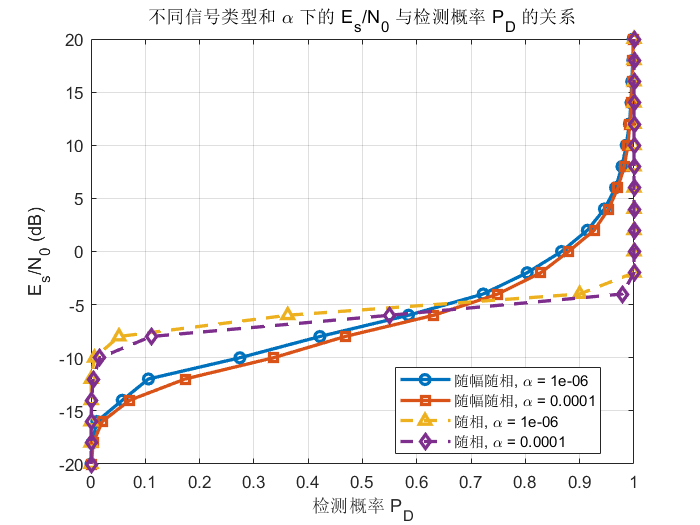
\includegraphics[width=0.7\textwidth]{image/output5.png}
    \caption{随幅随相信号和随相信号的检测性能曲线}
\end{figure}

从图中可以看出:

\begin{itemize}
    \item 随相信号在相同检测概率下通常比随幅随相信号所需的信噪比更低,表现出更优的抗噪性能。
    \item 随幅随相信号由于幅度的随机性,信号的能量分布更分散,导致在相同的检测概率下需要更高的信噪比。
\end{itemize}

\section*{五、鸢尾花分类预测}

\subsection*{1. 实验内容}

本实验旨在使用逻辑回归模型,对鸢尾花数据进行二分类预测,进而分析逻辑回归模型如何在分类问题中的应用。实验采用MindSpore作为深度学习框架,基于两类鸢尾花数据,构建逻辑回归模型并实现二分类预测。

实验主要可以分成以下几个步骤:
\begin{enumerate}
    \item 数据预处理:通过读取鸢尾花数据集,对数据进行预处理,包括数据清洗、数据标准化等。
    \item 模型构建与训练:使用MindSpore构建逻辑回归模型,并定义损失函数和优化器。通过在数据集上训练逻辑回归模型,并通过最小化损失函数学习模型参数。
    \item 模型评估:通过测试集对训练好的模型进行评估,计算模型的准确率,并进行可视化展示。
\end{enumerate}

\subsection*{2. 实验过程与结果}

\subsubsection*{数据预处理}

在数据预处理阶段,我们首先读取鸢尾花数据集,对数据进行清洗和标准化处理。数据集包含150个样本,每个样本包含4个特征(花萼长度、花萼宽度、花瓣长度、花瓣宽度)和1个标签(鸢尾花种类)。
我们将数据集按照 8:2 的比例划分为训练集和测试集,其中训练集用于模型训练,测试集用于模型评估。我们选取样本的前两种属性作为特征,标签作为类别进行二维可视化如图所示,可以看到基于前两种属性上的样本是线性可分的。

\begin{figure}[H]
    \centering
    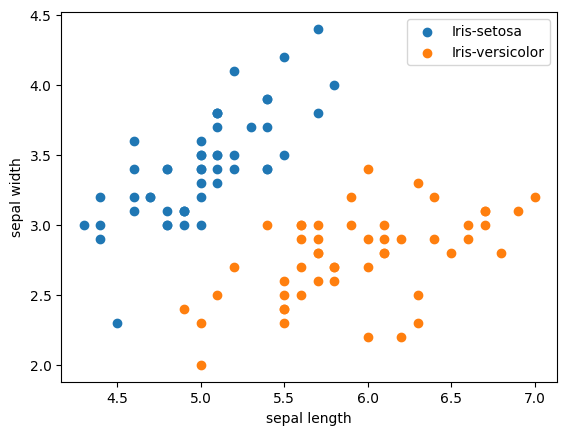
\includegraphics[width=0.7\textwidth]{image/output6.png}
    \caption{鸢尾花数据集二维可视化}
\end{figure}

\subsubsection*{模型构建与训练}

我们基于MindSpore框架定义逻辑回归模型,包含一个线性层和一个Sigmoid激活函数。定义损失函数为二元交叉熵损失函数,优化器为随机梯度下降(SGD)。
通过在训练集上迭代训练模型,最小化损失函数,学习模型参数。
对于每个样本\(N_i\),模型的计算方法如下:

\[ 
    Z_i = W \cdot X_i + b
\]
\[
    P_{i} = \text{sigmoid}(Z_{i}) = \frac{1}{1 + e^{-Z_{i}}} 
\]
\[
    \text{Loss} = -\frac{1}n\sum_i[Y_{i} * \log(P_{i}) + (1 - Y_{i})\log(1 - P_{i})]
\]


在模型训练部分,我们通过多次迭代epoch,用以更新模型参数,并观察loss的变化趋势,同时计算在测试集上的精度,直至结果收敛,且精度达到1为止,可认为结果满意。
通过绘制test数据的热力图如下所示,可以看到数据达到明显的线性可分效果。

\begin{figure}[H]
    \centering
    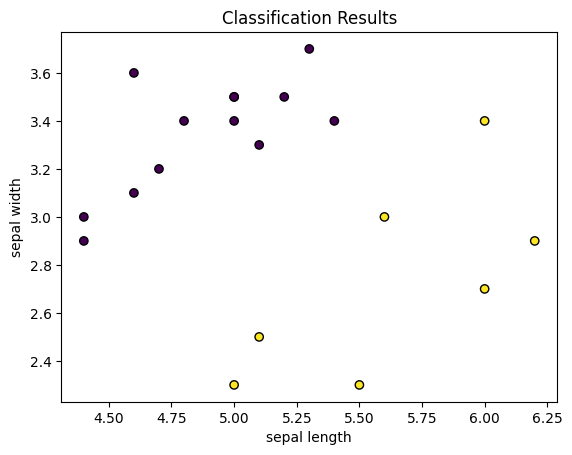
\includegraphics[width=0.7\textwidth]{image/output6-1.png}
    \caption{二分类分类结果热力图}
\end{figure}

\subsubsection*{创新设计}

在创新设计中,我们基于完整的Iris数据集,实现多分类任务。
与二分类实验类似,我们首先导入数据集并按照 8:2 的比例划分为训练集和测试集。按照标签的不同可以分成三类,其可视化如图所示。
图中我们可以看到,对于\texttt{Iris-versicolor}和\texttt{Iris-virginica}两类,二者在前两类下并不能通过线性分类进行较好的分类。

\begin{figure}[H]
    \centering
    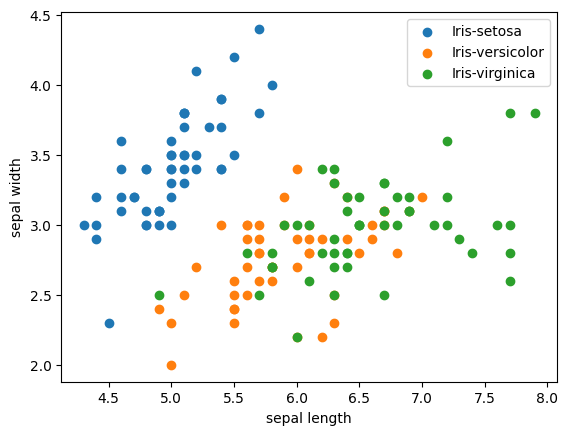
\includegraphics[width=0.7\textwidth]{image/output7.png}
    \caption{Iris数据集二维可视化-多分类}
\end{figure}

同样,我们通过基于MindSpore框架构建训练模型:
\begin{itemize}
    \item 模型构建:模型选用简单的全连接层,四输入三输出。模型选用Softmax将输出转换为概率分布,从而实现多分类任务。
    \item 损失函数:损失函数选用交叉熵损失函数,用于评估模型输出的概率分布与真实标签的差异。
    \item 优化方法:选用Momentum优化器,用于更新模型参数,并设置学习率为0.05。
    \item 训练过程:通过迭代25 epoch,用以更新模型参数,并观察loss的变化趋势,同时计算在测试集上的精度,直至结果收敛,且精度达到1为止,可认为结果满意。
\end{itemize}

同样绘制多分类任务的热力图如下所示,可以看到,在样本数据不能很好分类的部分数据,可以达到较为明显的线性可分效果。

\begin{figure}[H]
    \centering
    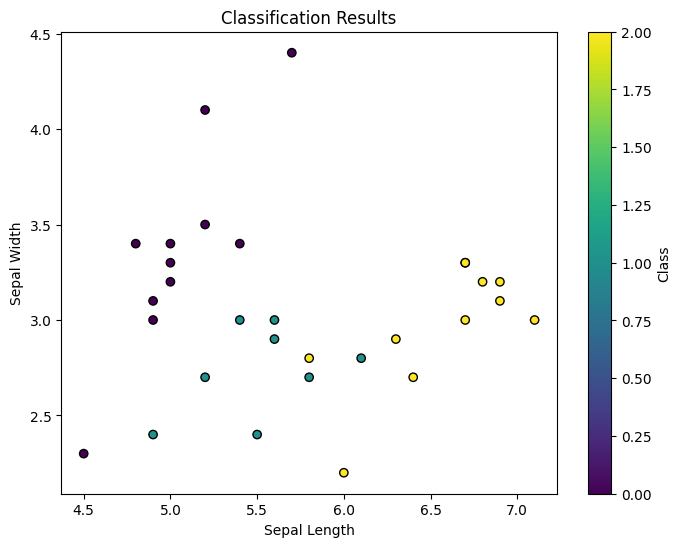
\includegraphics[width=0.7\textwidth]{image/output8.png}
    \caption{多分类分类结果热力图}
\end{figure}

\subsection*{3. 分析与讨论}

前面探讨的信号检测问题,本质上与这种分类问题也有着一些相似与不同,主要体现在其方法和目标存在部分差异:

\subsubsection*{相似点}

\begin{itemize}
    \item \textbf{二元判决}:在最基本的形式下,信号检测和分类问题都可以归结为二元判决问题(如信号检测中的“信号存在”或“信号不存在”,分类问题中的“类别 A”或“类别 B”)。
    \item \textbf{概率模型}:两者都可以使用概率模型来判断信号或类别的存在性。例如,分类问题中的逻辑回归和信号检测中的匹配滤波器都可以计算概率或相似度。
    \item \textbf{误判风险}:两者的最终目标都是在给定输入条件下,最小化错误判决(分类误差或误检率),以提高准确性和鲁棒性。
\end{itemize}

\subsubsection*{不同点}

\begin{itemize}
    \item \textbf{目标}:
    \begin{itemize}
        \item \textbf{信号检测}:信号检测的主要目的是判断特定信号是否存在,通常用于噪声背景中识别信号(例如雷达信号检测)。
        \item \textbf{分类问题}:分类的目标是根据输入特征将样本划分到不同的类别中,更多地关注数据的模式识别(如图像分类或文本分类)。
    \end{itemize}

    \item \textbf{输入数据特征}:
    \begin{itemize}
        \item \textbf{信号检测}:输入通常是一个时域或频域的连续信号,信号检测的关键是如何从噪声中提取信号特征。
        \item \textbf{分类问题}:输入通常是多维特征(向量或图像等),每个样本具有不同的特征维度,模型在特征空间中学习类别间的区别。
    \end{itemize}

    \item \textbf{决策方法}:
    \begin{itemize}
        \item \textbf{信号检测}:常用匹配滤波器、能量检测等方法,通过预设阈值判断信号是否存在,较多依赖物理特性。
        \item \textbf{分类问题}:分类问题多用机器学习方法,通过模型(如逻辑回归、决策树或神经网络)在特征空间中学习类别边界,更侧重于数据的统计特征。
    \end{itemize}

    
\end{itemize}

信号检测更关注信号在噪声背景中的存在性,而分类问题更关注多类之间的模式区分。
在机器学习的发展下,分类问题的技术也已逐渐应用于信号检测中,丰富了信号检测的方法选择。

\newpage

\begin{thebibliography}{99}

    \bibitem{Schonhoff2007}
    T.A. Schonhoff \& A.A. Giordano, \textit{Detection and Estimation: Theory and its Applications}. Pearson Education, Inc., 2007. (信号检测与估计——理论与应用,关欣等译,电子工业出版社,2012年).
    
    \bibitem{Srinath1996}
    M.D. Srinath, P.K. Rajasekaran \& R. Viswanathan, \textit{Introduction to Statistical Signal Processing with Applications}. Prentice Hall, 1996.  
    
    \bibitem{Kay1993}
    Steven M. Kay, \textit{Fundamentals of Statistical Signal Processing, Volume I: Estimation Theory} (©1993) \& \textit{Volume II: Detection Theory} (©1998). Pearson Education. (《统计信号处理基础:估计与检测理论(卷 I、卷 II合集)》,罗鹏飞等译,电子工业出版社,2023年).  
    
    \bibitem{Candy2016}
    James V. Candy, \textit{Bayesian Signal Processing: Classical, Modern, and Particle Filtering Methods} (2nd ed.). John Wiley \& Sons, Inc., 2016. (宗华等译,哈尔滨工业大学出版社,2023年).  
    
    \bibitem{VanTrees2013}
    Harry L. Van Trees, Kristine L. Bell, with Zhi Tian, \textit{Detection Estimation and Modulation Theory, Part I: Detection, Estimation, and Filtering Theory} (2nd ed.). John Wiley \& Sons, Inc., 2013.  
    
    \bibitem{ChatGPT2024}
    ChatGPT by OpenAI (2024). Personal communication and consultation for generating LaTeX formatting, experimental methodology, and model evaluation strategies. OpenAI, \url{https://www.openai.com}.  
    
\end{thebibliography}
    
    

\end{document}